\section{Durchführung}
Zunächst wird die sich in dem in Abbildung \ref{fig:aufb}
dargestellten Aufbau befindliche Probe über die Heizwicklung auf ca. $50° \text{C}$ erwärmt.\\
\begin{wrapfigure}{r}{7.0cm}
\fbox{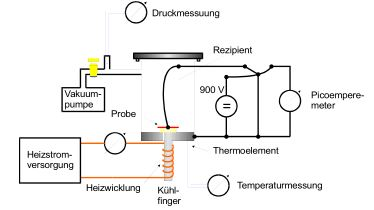
\includegraphics[width=7cm]{aufbau.JPG}}
\caption{Aufbau der Messvorrichtung \cite{V48}}
\label{fig:aufb}
\end{wrapfigure}
Ist diese Temperatur erreicht, wird mit der Ausrichtung der Dipole begonnen, indem mit dem Kondensator
ein elektrisches Feld erzeugt wird. Nach ca. 20 Minuten wird mit dem Einfrieren des Polarisationszustandes
begonnen,
indem die Probe mit flüssigem Stickstoff, welcher den Kühlfinger umgibt, auf $-60° \text{C}$ abgekühlt wird.
Zu sehen ist sowohl der Kühlfinger als auch die Heizspule in der rechts stehenden Abbildung in der Mitte unten.
Nachdem bei dieser Temperatur das E-Feld abgeschaltet und die Platten
durch Kurzschließen vollständig entladen sind, wird mit dem Aufheizen der Probe begonnen bis sie eine Temperatur von $60°\text{C}$ erreicht.
Dabei sollen Heizraten zwischen $\SI{1.5}{\celsius\per\minute}$ und $\SI{3.0}{\celsius\per\minute}$ gewählt werden. Jede Minute wird die Probentemperatur und
der Depolarisationsstrom von dem Thermometer und dem Picoamperemeter abgelesen.
Die Messung wird für zwei verschiedene Heizraten durchgeführt.
